\begin{frame}{RNA expression levels}
\label{sec:yeast_data}
\begin{columns}
\begin{column}{0.3\textwidth}

% RNA expression levels are gathered from TF, kinase and phosphatase mutant experiments. The TF mutant experiment data were collected from Luscombe et al.~\cite{Luscombe2010} which is based on the original experiments by Hu~et~al.~\cite{Hu2007}. Luscombe et al. improved upon the statistical work performed by Hu~et~al. by considering things like multiple testing problems. The kinase and phosphatase mutant experiments are from Holstege~et~al.~\cite{Holstege2010}. The TF mutants are derived from a BY4741 strain and the kinase/phosphatase mutant from a BY4742 strain.
\small
TF: Luscombe~et~al.~\cite{Luscombe2010}, \\ originally Hu~et~al.~\cite{Hu2007} \\
PK: Holstege~et~al.~\cite{Holstege2010} \\
Name conversion: Tiger~et~al.~\cite{Tiger2012}
\normalsize
% The measurements are gathered for cells at mid log-phase mainly on rich media, but some experiments were done with heat-stress and other stresses. Log-phase is the phase in a typical growth curve of a microorganism where the cells are increasing in number exponentially. The measurements are taken at this time in an attempt to have the cells observed under uniform reproducible conditions with expression levels and regulation as constant as possible.
% The RNA concentrations are measured for both wildtype and the strain under the experimental conditions which in this case are different knockout background. For most experiments a single gene is knocked out, but for some kinase and phosphatase experiments multiple genes have been knocked out.
% The measurements provided are log fold-change values, which are log-transformed ratios comparing the RNA concentration in a knockout experiment with the wildtype concentration~(\autoref{eq:logFC}).

\begin{equation}
\label{eq:logFC}
    x_i = \log_2 \left( \frac{x_i^{(\text{ko})}}{x_i^{(\text{wt})}} \right)
\end{equation}
% Here $x_i$ is the provided transformed value. The superscripts $(\text{ko})$ and $(\text{wt})$ indicates RNA measurements for knockout and wildtype experiment, respectively.
% The values are provided in a table for TF knockouts and another for PK knockouts, each having the knocked out gene indicated as column names and the gene for which RNA is measured indicated as row names. The names are given as popular names, as opposed to systematic names~(ORF~names).
% The log fold-change values are distributed around zero as a bell-curve with lighter tails than a normal distribution~(\autoref{fig:RNA_hist}). The means are $\mu_T \approx -0.023$ and $\mu_P \approx 0.0030$, and standard deviations $\sigma_T \approx 0.24$ and $\sigma_P \approx 0.17$ for transcription factor and kinase/phosphatase knockout experiments, respectively. We see that the majority of genes are not affected strongly be any random knockout.
% From Luscombe~et~al. there are 269 experiments each with a single transcription factor knockout. From Holstege~et~al. there are 144 experiments with a single kinase or phosphatase knockout, 16 with double kinase or phosphatase knockout and a single experiment with a triple knockout totaling at 161 experiments. 5 experiments from Luscombe have the same gene knocked out as from Holstege. An overview of counts can be found in~\autoref{tab:process_counts}.
\end{column}

\begin{column}{0.7\textwidth}
\begin{figure}[ht]
  \centering
  \begin{subfigure}[t]{0.49\textwidth}
  \centering
  \caption{}
  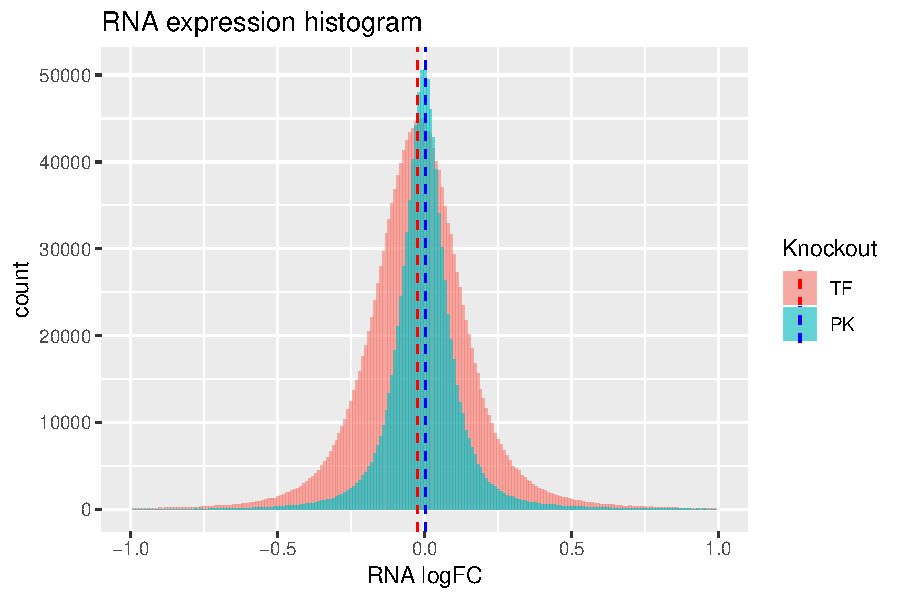
\includegraphics[width=\textwidth]{data/fig/RNA_hist.pdf}
  \label{fig:RNA_hist}
  \end{subfigure}
  \begin{subfigure}[t]{0.49\textwidth}
  \centering
  \caption{}
  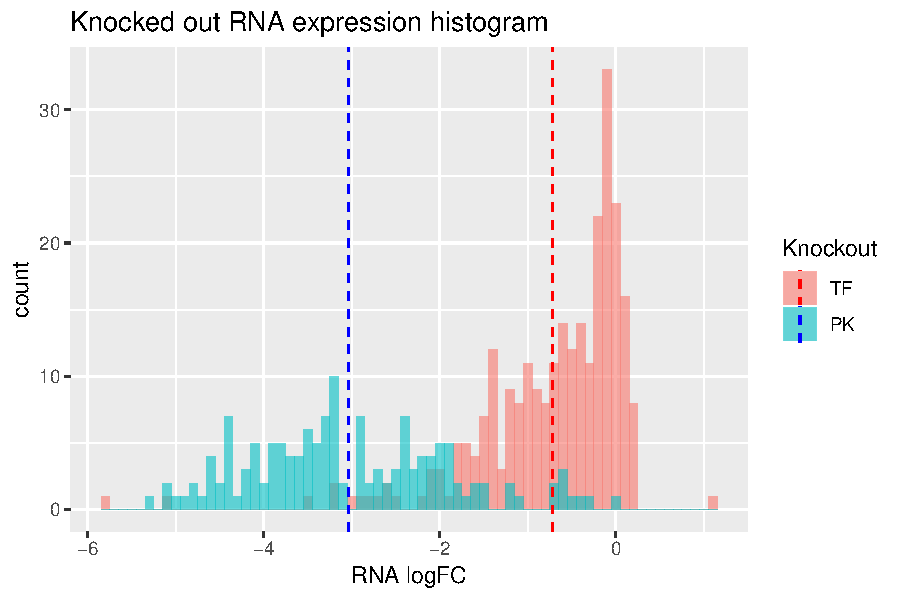
\includegraphics[width=\textwidth]{data/fig/knockout_RNA_hist.pdf}
  \label{fig:KO_RNA_hist}
  \end{subfigure}
  \caption{\textbf{RNA expression level histograms.} all (a) (TF: $269\cdot6253=\num{1.68e6}$, PK: $144\cdot6109=\num{0.88e6}$). Only KOs (b) (TF: 269, PK: 144). Dotted line = mean. }
\end{figure}
% Gene expression levels have been measured for all knockouts~(\autoref{fig:KO_RNA_hist}). The expression levels have mean $\mu_{T,KO} \approx -0.72$ and $\mu_{P,KO} \approx -3.0$ for transcription factor and kinase/phosphatase knockouts, respectively. As these are $\log_2$ fold-change values the means corresponds to a knocked out gene expressed ${\sim}1.6$ and ${\sim}8$ times less than wildtype for TF and PK, respectively.
\end{column}
\end{columns}
% Popular gene names were replaced with systematic names based on a conversion table from Tiger et al.~\cite{Tiger2012}.
% The simplest approach to format the data for use with the model is to filter it to enforce a perfect overlap in the genes for which log-fold change values are measured in the two datasets~(experiments with TF or PK knockouts). This makes it simple to concatenate measurements into a single matrix with known values at all entries.
% 
\small
\begin{table}[ht]
% \caption{\textbf{Protein types counted before and after preprocessing.} Counts of different types of proteins for which gene expression levels were measured. Counts are compared for raw data and data that has been filtered. TF KO, and PK KO refer to the work of Luscombe and Holstege, respectively. "PK and TF" refer to measurements of genes that are the intersection of the TF and PK sets and does therefore not add to the total. "neither" refers to genes that are never knocked out but still observed in the dataset. }
\begin{tabularx}{\textwidth}{@{}XXXXXX@{}}
    \toprule
    & TF & PK & PK and TF & neither & total \\
    \midrule
    TF KO & 269 & 144 & 5 & 5840 & 6253 \\
    PK KO & 266 & 144 & 5 & 5699 & 6109 \\
    processed & 266 & 144 & 5 & 5471 & 5881 \\
    \bottomrule
\end{tabularx}
\label{tab:process_counts}
\end{table}
\normalsize
% The filtering was performed, reducing the number of measured genes as described in \autoref{tab:process_counts}. Any measured gene is categorized as either a transcription factor, kinase/phosphatase, both or neither. We see that three TFs were not measured for kinase/phosphatase knockout experiments, which were removed both in terms of their knockout experiment as well as their expression level in knockout experiments of other transcription factors.

\end{frame}